\documentclass[14pt]{article}
\usepackage[utf8]{inputenc}
\usepackage[T2A]{fontenc}
\usepackage[russian]{babel}
\usepackage{amsmath, amssymb}
\usepackage{geometry}
\usepackage{graphicx}
\usepackage{xcolor}
\usepackage{hyperref}
\usepackage{tasks}
\usepackage{tcolorbox}
\tcbuselibrary{skins, breakable, theorems}
\usepackage{fancyhdr}
\usepackage{lastpage}
\usepackage{enumitem}
\usepackage{paracol} % Для многоколоночности
\usepackage{ifthen}
\usepackage{needspace}

% Определение команд для тангенса и котангенса (русский стиль)
\newcommand{\tg}{\operatorname{tg}}
\newcommand{\ctg}{\operatorname{ctg}}

% Настройка геометрии для более компактного вида (как в мобильных приложениях)
\geometry{a4paper, left=10mm, right=10mm, top=20mm, bottom=20mm, headheight=15pt}

% Цветовая палитра (более современные и мягкие цвета)
\definecolor{primary}{RGB}{52, 152, 219}       % Ярко-синий
\definecolor{secondary}{RGB}{46, 204, 113}     % Зеленый
\definecolor{accent}{RGB}{155, 89, 182}        % Фиолетовый
\definecolor{lightbg}{RGB}{248, 249, 250}      % Светло-серый фон
\definecolor{taskborder}{RGB}{230, 230, 230}   % Цвет границы задач
\definecolor{optionbg}{RGB}{240, 242, 245}     % Фон для вариантов ответа

% Основной фон страницы
\pagecolor{lightbg}

% Настройка гиперссылок
\hypersetup{
    colorlinks=true,
    linkcolor=primary,
    urlcolor=primary,
}

% Колонтитулы (более стильные)
\pagestyle{fancy}
\fancyhf{}
\fancyhead[L]{\textcolor{primary}{\textbf{MathCore | MOCK Test-7}}}
\fancyhead[R]{\textcolor{secondary}{Abdunazarov M.X.}}
\fancyfoot[L]{\href{https://t.me/Math_Core_Dtm_MS_Att}{\textcolor{primary}{MathCore}}}
\fancyfoot[R]{\href{https://t.me/Abd_mardon}{\textcolor{secondary}{@Abd\_mardon}}}
\fancyfoot[C]{\textcolor{gray}{\thepage/\pageref{LastPage}}}
\renewcommand{\headrulewidth}{0.5pt}
\renewcommand{\headrule}{\hbox to\headwidth{\color{primary}\leaders\hrule height \headrulewidth\hfill}}
\renewcommand{\footrulewidth}{0.5pt}
\renewcommand{\footrule}{\hbox to\headwidth{\color{secondary}\leaders\hrule height \footrulewidth\hfill}}

% Титульная страница (улучшенная)
\title{\Huge \textbf{\textcolor{primary}{MOCK Test-7}}}
\author{\textcolor{secondary}{Abdunazarov M.X.}}
\date{}

% Стиль для карточки вопроса
\newtcolorbox{questionbox}[2][]{
    enhanced,
    breakable,
    colback=white,
    colframe=primary,
    coltitle=white,
    fonttitle=\bfseries\large,
    title={Задача \hfill \textcolor{white}{#2}},
    attach boxed title to top left={xshift=5mm, yshift=-2mm},
    boxed title style={size=small, colback=primary, sharp corners},
    sharp corners,
    boxrule=0.5pt,
    left=5mm,
    right=5mm,
    top=5mm,
    bottom=5mm,
    drop fuzzy shadow,
    #1
}

% Стиль для вариантов ответов (как кнопки)
\newlist{options}{enumerate}{1}
\setlist[options]{
    label=\textbf{\Alph*)},
    leftmargin=*,
    itemsep=2pt,
    topsep=5pt,
    before={\vspace{2mm}\begin{tcolorbox}[
        colback=optionbg,
        colframe=white,
        sharp corners,
        boxrule=0pt,
        left=2mm,
        right=2mm,
        top=2mm,
        bottom=2mm,
    ]},
    after={\end{tcolorbox}\vspace{2mm}},
}

% Для рисунков (центрирование и тень)
\newcommand{\questionimage}[2][0.5\linewidth]{%
    \begin{center}
        \includegraphics[width=#1]{#2}
    \end{center}
}

% Для удобства: команда вставки вопроса с рисунком
\newcommand{\questionitem}[4]{%
    \needspace{5cm} % Предотвращает разрыв вопроса
    \begin{questionbox}{#1}
        #2
        \ifx&#3&% Если рисунок не пустой
        \else
            \questionimage{#3}
        \fi
        \begin{options}
            #4
        \end{options}
    \end{questionbox}
}

\begin{document}

% Титульная страница
\maketitle
\begin{center}
    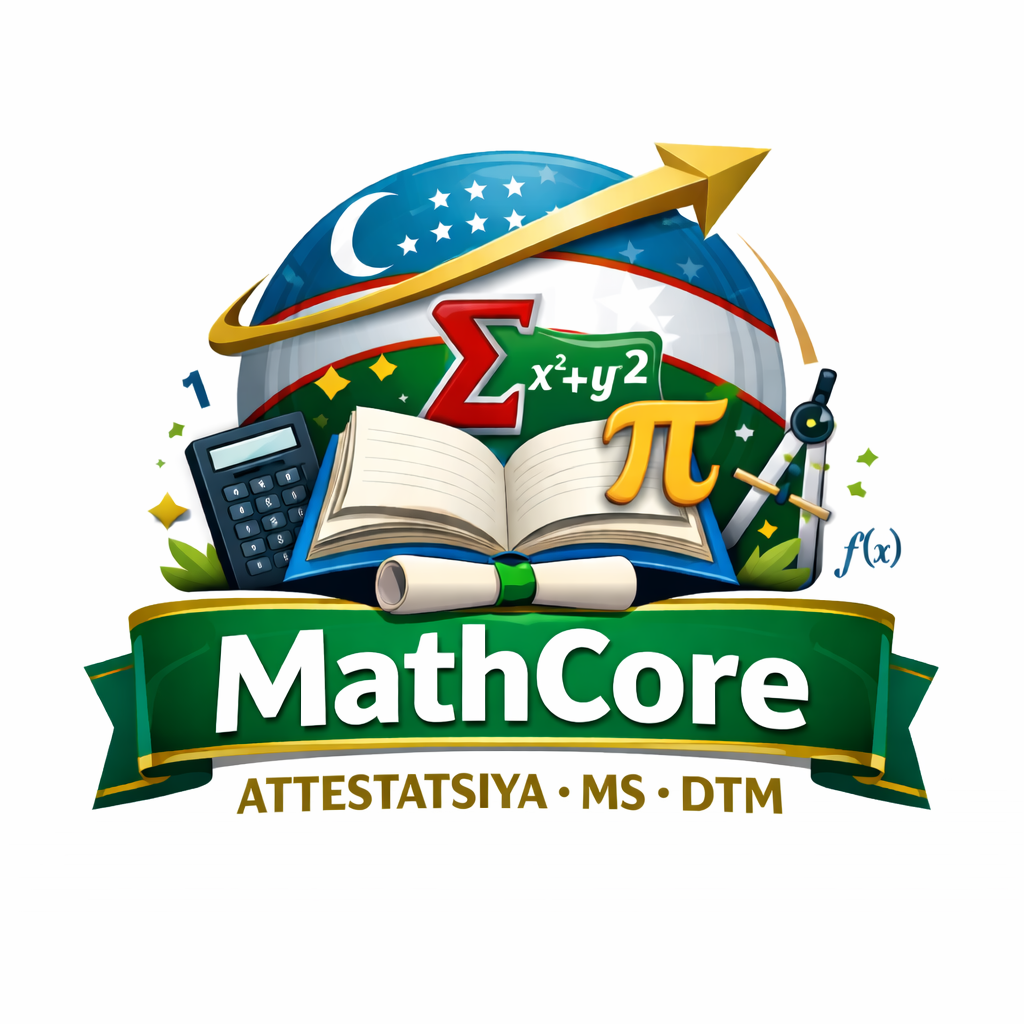
\includegraphics[width=0.2\textwidth]{logo.png} \\[5mm]
    \textcolor{gray}{\small Telegram: \href{https://t.me/Math_Core_Dtm_MS_Att}{@Math\_Core\_Dtm\_MS\_Att}}
\end{center}
\vspace{5mm}

% Задача 1
\begin{questionbox}{1}
    Если \(f(x)\) — убывающая функция, \(g(x)\) — возрастающая функция и \(x_1 < x_2 < x_3 < x_4\), 
    \(f(x_1) - f(x_2) = a\), \(g(x_3) - g(x_4) = b\), то какое из следующих утверждений верно?
    \begin{options}
        \item \(a \cdot b > 0\)
        \item \(a + b < 0\)
        \item \(-a + b > 0\)
        \item \(a > 0 > b\)
    \end{options}
\end{questionbox}

% Задача 2
\begin{questionbox}{2}
    Если \(5 + 6 + 7 + 8 + 9 + \cdots + n = 290\), то \(n = ?\)
    \begin{options}
        \item 36
        \item 24
        \item 32
        \item 28
    \end{options}
\end{questionbox}

% Задача 3
\begin{questionbox}{3}
    Для двузначного числа \(x\) выполняется \(\text{НОД}(x, 13) = 1\). Найдите максимальное произведение цифр числа \(x\).
    \begin{options}
        \item 81
        \item 69
        \item 75
        \item 85
    \end{options}
\end{questionbox}

% Задача 4
\begin{questionbox}{4}
    Найдите остаток от деления \(7 \cdot 7^{15}\) на 8.
    \begin{options}
        \item 1
        \item 7
        \item 3
        \item 6
    \end{options}
\end{questionbox}

% Задача 5
\begin{questionbox}{5}
    При каком значении \(m\) выражение \(x(x + a)(x + b)(x + a + b) + 25m^2\) является полным квадратом?
    \begin{options}
        \item \(\pm \frac{ab}{5}\)
        \item \(\pm \frac{ab}{10}\)
        \item \(\pm ab\)
        \item \(\pm \frac{ab}{4}\)
    \end{options}
\end{questionbox}

% Задача 6
\begin{questionbox}{6}
    Если \(x^2 - x = 3\), то найдите значение \(\frac{x^2 -3}{x^2+x-3}\)? 
    \begin{options}
        \item \(-\frac{1}{2}\)
        \item \(-\frac{1}{3}\)
        \item \(1\)
        \item \(\frac{1}{2}\)
    \end{options}
\end{questionbox}

% Задача 7
\begin{questionbox}{7}
    Решите неравенство \(x^{\lg^2 x - 3\lg x + 1} < 1000\).
    \begin{options}
        \item \((0; 100)\)
        \item \((0; 1000)\)
        \item \((10; 100)\)
        \item \((100; 1000)\)
    \end{options}
\end{questionbox}

% Задача 8
\begin{questionbox}{8}
    В геометрической прогрессии, состоящей из 6 членов, сумма первых трех членов равна 26, а сумма последних трех членов равна 702. Найдите знаменатель прогрессии.
    \begin{options}
        \item 8
        \item 6
        \item 2
        \item 3
    \end{options}
\end{questionbox}

% Задача 9
\begin{questionbox}{9}
    Сколько целых чисел удовлетворяет неравенству \(3\sqrt{5-x} \le (x-4)\ln(x-4)\)?
    \begin{options}
        \item \(\varnothing\)
        \item 2
        \item 1
        \item 3
    \end{options}
\end{questionbox}

% Задача 10
\begin{questionbox}{10}
    Найдите решения неравенства \(\left(x - \frac{\pi}{6}\right)\left(\sin x - \frac{1}{2}\right) > 0\) на промежутке \([0; 2\pi]\).
    \begin{options}
        \item \(\left[0; \frac{\pi}{6}\right]\)
        \item \(\left(\frac{\pi}{6}; \frac{5\pi}{6}\right)\)
        \item \(\left(\frac{\pi}{6}; \frac{\pi}{3}\right)\)
        \item \(\left(0; \frac{\pi}{6}\right) \cup \left(\frac{\pi}{6}; \frac{5\pi}{6}\right)\)
    \end{options}
\end{questionbox}

% Задача 11
\begin{questionbox}{11}
    Вычислите \(\arctg 1 + \arctg 2 + \arctg 3\).
    \begin{options}
        \item \(\frac{\pi}{2}\)
        \item \(\pi\)
        \item \(\frac{3\pi}{2}\)
        \item \(2\pi\)
    \end{options}
\end{questionbox}

% Задача 12
\begin{questionbox}{12}
   В библиотеке имеется 4 вида книг, причём экземпляров каждого вида достаточно много. Сколькими способами можно выбрать 5 книг?
    \begin{options}
        \item \(56\)
        \item \(4^5\)
        \item \(5^4\)
        \item 20
    \end{options}
\end{questionbox}

% Задача 13
\begin{questionbox}{13}
    Монету подбрасывают 5 раз. Найдите вероятность того, что решка (сторона с номиналом) выпадет ровно 3 раза.
    \begin{options}
        \item \(\frac{5}{32}\)
        \item \(\frac{5}{16}\)
        \item \(\frac{7}{32}\)
        \item \(\frac{1}{32}\)
    \end{options}
\end{questionbox}

% Задача 14 (исправлено дублирование)
\begin{questionbox}{14}
    Найдите свободный член выражения \((x^3 + \frac{1}{\sqrt{x}})^{14}\)? 
    \begin{options}
        \item 50
        \item 45
        \item 91
        \item 84
    \end{options}
\end{questionbox}

% Задача 15
\begin{questionbox}{15}
    В ящике 10 шаров, пронумерованных от 1 до 10. Из ящика случайно выбирают два шара. Известно, что сумма номеров выбранных шаров равна 14. Какова вероятность того, что был выбран шар с номером 6?
    \begin{options}
        \item \(\frac{1}{3}\)
        \item \(\frac{1}{6}\)
        \item \(\frac{1}{2}\)
        \item \(\frac{2}{3}\)
        \item \(\frac{5}{6}\)
    \end{options}
\end{questionbox}

% Задача 16
\begin{questionbox}{16}
    Дана функция \(h(x) = \frac{f(3x)}{g(2x)}\). Известно, что \(f(3) = 2\), \(g(2) = 3\), \(f'(3) = 4\) и \(g'(2) = 5\) если \(g(2x)\). Чему равно \(h'(1)\)?
    \begin{options}
        \item \(\frac{9}{16}\)
        \item \(\frac{2}{3}\)
        \item \(\frac{16}{9}\)
        \item \(\frac{3}{4}\)
    \end{options}
\end{questionbox}

% Задача 17
\begin{questionbox}{17}
    На рисунке изображен график функции \(y = x^3\). Точка \(x=1\) принадлежит этой функции. Найдите площадь закрашенной области.
   \begin{center}
       \centering
       
\includegraphics[width=0.4\linewidth]{1.png}
   \end{center}
    \begin{options}
        \item \(\frac{3}{2}\)
        \item \(\frac{1}{3}\)
        \item \(\frac{1}{6}\)
        \item \(\frac{1}{2}\)
    \end{options}
\end{questionbox}

% Задача 18
\begin{questionbox}{18}
    Вычислите интеграл \(\displaystyle \int \tg^2 x \, dx + \int \tg^4 x \, dx\).
    \begin{options}
        \item \(\frac{1}{3} \tg^2 x + C\)
        \item \(x + 3\tg^2 x + C\)
        \item \(3x + \tg x + C\)
        \item \(\frac{1}{3} \tg^3 x + C\)
    \end{options}
\end{questionbox}

% Задача 19
\begin{questionbox}{19}
    Если \(f(x+2) = f(x) + x\) и \(f(2) = 3\), то найдите \(f(8)\).
    \begin{options}
        \item 15
        \item 9
        \item 12
        \item 10
    \end{options}
\end{questionbox}

% Задача 20
\begin{questionbox}{20}
    Вычислите: \(\displaystyle \int_{-1}^{0} \frac{e^{2x} - 2}{e^x} \, dx\).
    \begin{options}
        \item \(2e - \frac{1}{e}\)
        \item \(2e + 3\)
        \item \(2e + \frac{1}{e} - 3\)
        \item \(\frac{3e - 2e^2 - 1}{e}\)
    \end{options}
\end{questionbox}

% Задача 21
\begin{questionbox}{21}
    Используя предоставленные данные, найдите площадь закрашенной области.
    \begin{center}
        \begin{center}
            \centering
            
\includegraphics[width=0.3\linewidth]{2.png}
        \end{center}
    \end{center}
    \begin{options}
        \item \(\frac{14}{3}\)
        \item \(\frac{16}{3}\)
        \item \(\frac{10}{2}\)
        \item \(\frac{17}{3}\)
    \end{options}
\end{questionbox}

% Задача 22
\begin{questionbox}{22}
    Сколько из следующих утверждений неверны?
    \begin{enumerate}[label=\arabic*.]
        \item Если стороны треугольника равны 4, 6 и 9, то его периметр равен 19;
        \item Если при пересечении двух прямых третьей внутренние накрест лежащие углы равны, то эти прямые параллельны;
        \item Центр окружности, вписанной в треугольник, лежит в точке пересечения биссектрис;
        \item Радиус окружности, вписанной в любой правильный многоугольник, равен \(R = \dfrac{a}{2 \sin \frac{180^\circ}{n}}\) (где \(a\) — сторона многоугольника, \(n\) — количество сторон).
    \end{enumerate}
    \begin{options}
        \item 1
        \item 3
        \item 2
        \item 4
    \end{options}
\end{questionbox}

% Задача 23
\begin{questionbox}{23}
    В трапеции при пересечении диагоналей образовались треугольники. Известно, что \(S_{\triangle AED} = 8\) и \(S_{\triangle DEC} = 4\). Найдите площадь закрашенной области.
    \begin{center}
       
\includegraphics[width=0.3\linewidth]{3.png}
    \end{center}
    \begin{options}
         \item 24
        \item 12
        \item 16
        \item 14
    \end{options}
\end{questionbox}

% Задача 24
\begin{questionbox}{24}
    Стороны треугольника разделены точками, начиная от вершин, в отношении \(3:5:7\). Через точки деления проведены прямые, параллельные основанию. Найдите отношение площадей полученных фигур.
    \begin{options}
        \item \(3: 5: 7\)
        \item \(9: 25: 49\)
        \item \(9: 64: 225\)
        \item \(9: 55: 161\)
    \end{options}
\end{questionbox}

% Задача 25
\begin{questionbox}{25}
    На рисунке даны прямоугольные треугольники ABC и ADC (DE \(\perp\) AC). Используя предоставленные данные, найдите x.
    \begin{center}
        
\includegraphics[width=0.3\linewidth]{4.png}
    \end{center}
    \begin{options}
        \item \(16\)
        \item \(20\)
        \item \(8\sqrt{2}\)
        \item \(16\sqrt{2}\)
    \end{options}
\end{questionbox}


% Задача 26
\begin{questionbox}{26}
   Найдите значение \(S_1 - S_2\).
   \begin{center}
       \centering
       
\includegraphics[width=0.3\linewidth]{5.png}
   \end{center}
    \begin{options}
        \item \(2\pi\)
        \item \(4\pi\)
        \item \(3\pi\)
        \item \(6\pi\)
    \end{options}
\end{questionbox}

% Задача 27
\begin{questionbox}{27}
    Дан параллелограмм ABCD с векторами \(\overrightarrow{AB}(3; 5; -7)\) и \(\overrightarrow{AD}(-11; 7; 3)\). O — точка пересечения диагоналей параллелограмма. Найдите сумму координат вектора \(\overrightarrow{OD}\).
    \begin{options}
        \item 1
        \item 0
        \item -1
        \item 2
    \end{options}
\end{questionbox}

% Задача 28
\begin{questionbox}{28}
    В прямоугольнике ABCD на рисунке \(S_{\triangle AOD}=30\) и \(S_{\triangle BOC}=50\) и \(DC=16\). Найдите длину стороны AD.
    \begin{center}
        
\includegraphics[width=0.3\linewidth]{6.png}
    \end{center}
    \begin{options}
        \item 10
        \item 45
        \item 15
        \item 40
    \end{options}
\end{questionbox}

% Задача 29
\begin{questionbox}{29}
    К полуокружности с центром в точке O проведена касательная в точке D. Основываясь на предоставленных данных, найдите OD.
    \begin{center}
         
\includegraphics[width=0.5\linewidth]{7.png}
    \end{center}
    \begin{options}
        \item 2
        \item 6
        \item 4
        \item 3
    \end{options}
\end{questionbox}

% Задача 30
\begin{questionbox}{30}
    На рисунке изображены кубики с ребром, равным 1. Чему равна длина вдоль линии, обозначенной пунктиром?
    \begin{center}
         
\includegraphics[width=0.5\linewidth]{8.png}
    \end{center}
    \begin{options}
        \item \(\sqrt{13}\)
        \item \(\sqrt{12}\)
        \item \(\sqrt{14}\)
        \item \(\sqrt{17}\)
        
        
    \end{options}
\end{questionbox}

% Задача 31
\begin{questionbox}{31}
    Даны точки \(K(0, 7)\) и \(L(1, 0)\). Найдите объем тела, полученного при вращении отрезка \(KL\) вокруг оси \(Oy\) на угол \(90^\circ\).
    \begin{center}
        \centering
        
\includegraphics[width=0.3\linewidth]{9.png}
    \end{center}
    \begin{options}
        \item \(\frac{7\pi}{6}\)
        \item \(\frac{7\pi}{3}\)
        \item \(\frac{7\pi}{12}\)
        \item \(\frac{9\pi}{4}\)
        
    \end{options}
\end{questionbox}

% Задача 32
\begin{questionbox}{32}
   Чему равен объем тела, полученного при вращении области, ограниченной осью $x$ и линиями \(x-y+4=0\) и \(x-2y+8=0\) , вокруг оси $y$ на 360°?
    
    \begin{options}
        \item \(32\pi\)
        \item \(48\pi\)
        \item \(54\pi\)
        \item \(64\pi\)
    \end{options}
\end{questionbox}

% Задача 33
\begin{questionbox}{33}
    Если \(AD=22\), \(BE=16\), \(EF=12\) и \(KF=7\), найдите длину отрезка \(PL\).
    \begin{center}
        
\includegraphics[width=0.3\linewidth]{12.png}
    \end{center}
    \begin{options}
        \item 26
        \item 30
        \item 25
        \item 27
    \end{options}
\end{questionbox}

% Задача 34
\begin{questionbox}{34}
    Гипотенуза прямоугольного треугольника равна 12. Дана точка, находящаяся на расстоянии 10 от всех вершин треугольника и расположенная вне его плоскости. Найдите расстояние от этой точки до плоскости треугольника.
    \begin{options}
        \item 8
        \item 10
        \item \(\sqrt{44}\)
        \item 12
    \end{options}
\end{questionbox}

% Задача 35
\begin{questionbox}{35}
    Объем конуса равен \(3\pi\) м\(^3\). Если развертка его боковой поверхности представляет собой полукруг, найдите площадь полной поверхности конуса.
    \begin{options}
        \item \(6\pi\)
        \item \(2\pi\)
        \item \(9\pi\)
        \item \(18\pi\)
    \end{options}
\end{questionbox}

\end{document}